\subsection{Refactoring the Drawer Layout}
The behaviour of the original drawer, described in \cref{sec:drawer:behaviour}, has the unfortunate effect of pushing the applications icons to the right, as the drawer is dragged open.
This is caused by the view containing the application icons having the  \lstinline{android:layout_toRightOf} attribute set to be placed to the right of the sidebar in the layout XML files.
This makes its position adjust automatically to the newest rightmost position of the sidebar each time the bar is moved, effectively pushing the icons off the screen.

The main issue with the current implementation of the \homeactivity layout lies in the fact that many parameters such as heights and widths are set at compile-time through constants.
The result is that the layout does not adapt to other devices than the one it has been designed for, which is not viable if the customers choose to replace their current ones.
The improved implementation includes restructuring all parts of the XML file defining the layout of the \homeactivity, making it adapt to devices with various screen sizes and pixel density.

\subsubsection{Implementation}\label{sec:sidebarlayout:xml}
To avoid the icons being pushed outside the screen, the layout for the drawer is restructured so its elements are contained within a custom view called \lstinline|DrawerLayout|.
This ensures that the animation and layout hierarchy can be controlled more effectively, making the drawer being drawn on top of other layout elements.

\Cref{lst:sidebarlayout} shows the elements of the XML layout.

\begin{lstlisting}[caption={Structure of the XML layout of the drawer. Note that some attributes are omitted.},label={lst:sidebarlayout}, language=XML]
<dk.aau.cs.giraf.launcher.layoutcontroller.DrawerLayout android:id="@+id/DrawerView" android:layout_marginLeft="-400dp">

<RelativeLayout android:id="@+id/DrawerContentView" android:layout_width="400dp">
<GridView android:id="@+id/appcolors" />
</RelativeLayout>

<RelativeLayout android:id="@+id/SidebarView">
<dk.aau.cs.giraf.gui.GWidgetProfileSelection />
<dk.aau.cs.giraf.gui.GButtonSettings />
<dk.aau.cs.giraf.gui.GWidgetLogout />
</RelativeLayout>

</dk.aau.cs.giraf.launcher.layoutcontroller.DrawerLayout>

<ScrollView android:id="@+id/appScrollView"/>
\end{lstlisting}

Notice the \lstinline|ScrollView| on the last line in \Cref{lst:sidebarlayout}.
The before mentioned \lstinline{android:layout_toRightOf} attribute on this \lstinline|ScrollView| has been removed, to keep it from being pushed out of the screen.
The margin of $-400dp$ defined on Line 1 effectively hides the \lstinline|SideBarLayout| when the \homeactivity has just started, revealing only the \lstinline|SideBar|.
Since the \lstinline|SideBar| is placed next to the \lstinline|GridView| and this view has the width of the margin defined on \lstinline|SideBarLayout|, it is the only visible element.
This gives the impression of a closed drawer, and is illustrated in \cref{fig:drawerhidden}.

\begin{figure}[h]
\centering
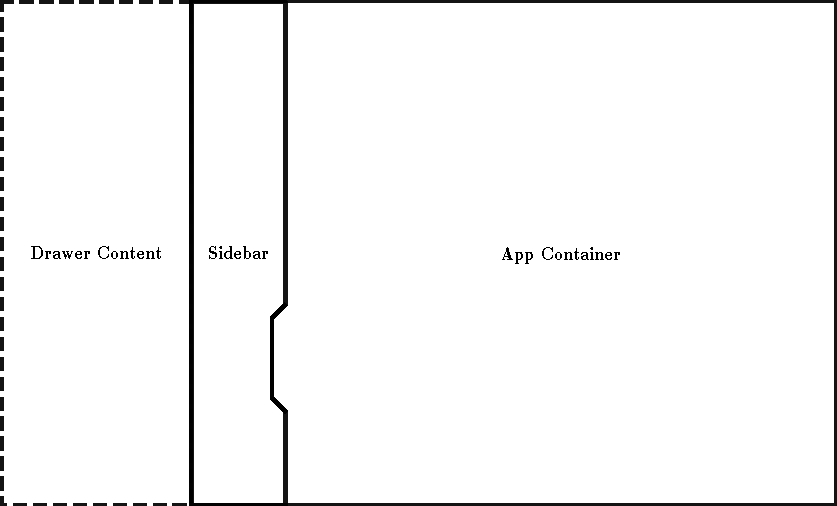
\includegraphics[width=\textwidth]{drawer.pdf}
\caption{The layout of the drawer when it is closed. This dashed lines represent parts of the drawer that is not visible to the used.}
\label{fig:drawerhidden}
\end{figure}